\documentclass{article}
\usepackage{amsmath, amssymb, graphicx}
\usepackage[margin=1in]{geometry}
\usepackage{booktabs}
\usepackage{siunitx}
\usepackage{hyperref}
\usepackage{listings}
\usepackage{xcolor}

\sisetup{group-separator={,}, group-minimum-digits=4}
\lstset{
  basicstyle=\ttfamily\footnotesize,
  breaklines=true,
  frame=single,
  keywordstyle=\color{blue!60!black},
  commentstyle=\color{green!40!black},
  showstringspaces=false
}

\title{Classical and CCE-QUBO Foundations for Quantum-Assisted NPU Scheduling}
\author{}
\date{}

\begin{document}
\maketitle

\begin{abstract}
Neural processing units are increasingly constrained by scheduling quality rather than nominal peak throughput, because effective performance depends on tightly coupled compute, memory, and control decisions. We present the classical foundation of a constraint-coupled energy formulation, CCE-QUBO, that models NPU scheduling as a binary quadratic program with unary, pairwise, higher-order, and feasibility penalty terms. In our evaluation we observe consistent gains over a strong greedy baseline on representative small (10-node), medium (25-node), and large (42-node) operator graphs under multi-level memory and bandwidth limits. On the medium workload, CCE-QUBO reduces average cost from 1120 to 902 (19.5\% improvement), and CCE-QUBO with adaptive penalty refinement (APR) further reduces cost to 842 (24.8\% improvement) while improving feasibility from 82.1\% to 96.7\%. Latency decreases from 15,840 to 13,110 cycles (17.2\%), and DRAM traffic drops from 8.9 to 6.8 GB (23.6\%). Ablation analysis shows that removing higher-order terms or APR significantly degrades both feasibility and stall behavior, confirming that cross-term modeling is necessary beyond additive objectives. The resulting pipeline is solver-agnostic and directly compatible with a QAOA backend, enabling controlled classical-to-quantum integration without objective mismatch.
\end{abstract}

\section{Introduction}
NPU schedulers operate under interacting constraints: finite compute resources, strict operator dependencies, hierarchical memories, bursty DRAM behavior, and optional DVFS control. Practical bottlenecks emerge when local scheduling choices induce non-local effects such as SRAM eviction cascades, bandwidth spikes, and idle pipeline slots. These effects are weakly captured by additive heuristic scores.

Conventional cost-based schedulers and fixed-penalty formulations are attractive for speed, but they often under-represent interaction structure and can be brittle under changing workload or hardware regimes. We therefore model scheduling as an energy minimization problem where interaction terms and feasibility penalties are first-class components.

Our approach combines CCE-QUBO construction with a classical optimization stack and APR-based penalty adaptation, then exposes a clean interface for quantum solvers. The objective is not to append quantum routines to a heuristic scheduler, but to define a unified optimization problem that classical and quantum methods both optimize.

\noindent\textbf{Contributions.}
\begin{itemize}
\item We formalize CCE-QUBO for NPU scheduling with explicit unary, pairwise, higher-order, and constraint components.
\item We build a classical pipeline (greedy, lookahead, beam, annealing) coupled with APR for stable feasibility improvement.
\item We provide a quantitative experimental study with multi-seed evaluation, detailed energy decomposition, and targeted ablations.
\item We maintain a solver-agnostic interface so the same QUBO instances can be consumed by a QAOA backend.
\end{itemize}

\section{Problem Setup}
Let $G=(V,E)$ denote an operator DAG with $|V|=N$ operators and precedence edges $(i,j)\in E$. Scheduling occurs over a discrete horizon $\mathcal{T}=\{0,\dots,T-1\}$, resources $\mathcal{R}$, memory levels $\mathcal{L}$ (e.g., L1, L2, DRAM), and DVFS states $\mathcal{F}$. A schedule must satisfy precedence, resource compatibility, memory capacity, and DVFS validity constraints while minimizing performance cost.

Workloads are CNN/transformer-derived DAGs with heterogeneous operator sizes and fanout patterns. The hardware model includes multiple execution resources, finite SRAM banks, DRAM bandwidth ceilings, and per-state DVFS energy factors. This setup intentionally stresses cross-term interactions between compute placement, temporal alignment, and memory traffic.

\begin{table}[t]
\centering
\caption{Notation used throughout the classical and quantum documents.}
\begin{tabular}{ll}
\toprule
Symbol & Description \\
\midrule
$i,j$ & Operator indices in $V$ \\
$t$ & Discrete time slot index in $\mathcal{T}$ \\
$r$ & Compute resource index in $\mathcal{R}$ \\
$\ell$ & Memory level index in $\mathcal{L}$ \\
$s$ & DVFS state index in $\mathcal{F}$ \\
$x_{i,t,r}$ & 1 iff operator $i$ executes at $(t,r)$ \\
$m_{i,\ell}$ & 1 iff operator $i$ uses memory level $\ell$ \\
$f_{t,s}$ & 1 iff DVFS state $s$ is active at time $t$ \\
$u_{b,t}$ & Auxiliary bank-congestion indicator for bank $b$, time $t$ \\
$v_t$ & Auxiliary burst-congestion indicator at time $t$ \\
$\lambda_k$ & Penalty weight for constraint family $k$ \\
$\alpha,\beta,\gamma$ & Weights for unary, pairwise, and higher-order terms \\
\bottomrule
\end{tabular}
\end{table}

\section{CCE-QUBO Formulation}
We define binary vector $\mathbf{z}\in\{0,1\}^n$ collecting all decision and auxiliary variables. The total objective is
\begin{equation}
E(\mathbf{z}) = E_{\text{unary}}(\mathbf{z}) + E_{\text{pair}}(\mathbf{z}) + E_{\text{high}}(\mathbf{z}) + E_{\text{constr}}(\mathbf{z};\lambda).
\end{equation}
The final solver form is
\begin{equation}
E(\mathbf{z}) = c + \sum_{i=1}^{n} a_i z_i + \sum_{1\le i\le j\le n} b_{ij} z_i z_j.
\end{equation}

\subsection{Unary Terms}
Unary terms capture local execution and state costs:
\begin{align}
E_{\text{unary}} =
&\;\alpha_{\mathrm{comp}}\sum_{i,t,r} c^{\mathrm{comp}}_{i,r}x_{i,t,r}
+ \alpha_{\mathrm{energy}}\sum_{i,\ell} c^{\mathrm{mem}}_{i,\ell}m_{i,\ell} \\
&+ \alpha_{\mathrm{lat}}\sum_{i,t,r} c^{\mathrm{lat}}_{i,t}x_{i,t,r}
+ \alpha_{\mathrm{dvfs}}\sum_{t,s} c^{\mathrm{dvfs}}_{t,s}f_{t,s}.
\end{align}
The terms encode compute effort, DRAM/SRAM access energy, latency pressure, and DVFS state cost.

\subsection{Pairwise Terms}
Pairwise interactions encode reuse, fusion, and bandwidth coupling:
\begin{align}
E_{\text{pair}} =
&\;\beta_{\mathrm{reuse}}\sum_{(i,j)}\sum_{t,t',r} w^{\mathrm{reuse}}_{ijtt'r}x_{i,t,r}x_{j,t',r} \\
&+ \beta_{\mathrm{fuse}}\sum_{(i,j)}\sum_{t,r} w^{\mathrm{fuse}}_{ijtr}x_{i,t,r}x_{j,t+1,r}
+ \beta_{\mathrm{bw}}\sum_{(i,j)}\sum_{t,r,r'} w^{\mathrm{bw}}_{ijtrr'}x_{i,t,r}x_{j,t,r'}.
\end{align}
Reuse and fusion introduce favorable couplings for temporally aligned operators, while bandwidth terms penalize harmful overlap.

\subsection{Higher-Order Effects via Auxiliary Variables}
Higher-order terms are approximated through auxiliary variables with quadratic tie constraints. For bank conflicts:
\begin{equation}
E_{\mathrm{bank}} = \gamma_{\mathrm{bank}}\sum_{b,t}u_{b,t} + \rho_{\mathrm{bank}}\sum_{b,t}\left(\sum_{i,r} a_{i,r,b}x_{i,t,r} - \theta_b u_{b,t}\right)^2.
\end{equation}
For burst congestion over window $\mathcal{W}(t)$:
\begin{equation}
E_{\mathrm{burst}} = \gamma_{\mathrm{burst}}\sum_t v_t + \rho_{\mathrm{burst}}\sum_t\left(\sum_{\tau\in\mathcal{W}(t)}\sum_{i,r} d_i x_{i,\tau,r} - \kappa v_t\right)^2.
\end{equation}
Stall cascades and parallelism collapse are encoded analogously with additional auxiliaries tied to serialized-ready patterns and sustained backlog indicators.

\subsection{Constraint Penalties}
Constraint penalties are
\begin{equation}
E_{\text{constr}}(\mathbf{z};\lambda) = \sum_k \lambda_k C_k(\mathbf{z}).
\end{equation}
Representative constraints include
\begin{align}
C_{\mathrm{unique}} &= \sum_i \left(\sum_{t,r}x_{i,t,r}-1\right)^2, \\
C_{\mathrm{dep}} &= \sum_{(i,j)\in E}\sum_{t_i,t_j}\mathbf{1}[t_j < t_i + d_i] \sum_{r,r'}x_{i,t_i,r}x_{j,t_j,r'}, \\
C_{\mathrm{dvfs}} &= \sum_t\left(\sum_s f_{t,s}-1\right)^2,
\end{align}
with memory-capacity penalties applied per time and memory level using bind auxiliaries between $x_{i,t,r}$ and $m_{i,\ell}$.

\section{Experimental Setup}
The experiment harness in \texttt{run\_experiment.py} evaluates multiple workloads and methods under identical hardware assumptions. We use three graph-size regimes: small (10 operators), medium (25 operators), and large (42 operators), each with 5--10 random seeds per method. The medium case reported in detail below corresponds to a branch-heavy CNN-derived DAG.

Hardware assumptions include 2 NPU resources, 3 memory levels (L1/L2/DRAM), 3 DVFS states, 6 SRAM banks, and finite per-slot DRAM bandwidth. Methods are: greedy baseline, CCE-QUBO without APR, and CCE-QUBO with APR. CCE optimization uses beam width 5 for constructive search, simulated annealing with 320 iterations, start temperature 3.8, end temperature 0.04, and APR rounds of 8 with clipped updates.

Metrics are computed from schedule execution and model instrumentation: total cost, latency cycles, DRAM traffic, bandwidth utilization, stall cycles, feasibility percentage, and wall-clock runtime. Means and standard deviations are computed across seeds.

\section{Results}
\subsection{Main Results Table}
Table~\ref{tab:main-medium} reports medium-workload performance. CCE-QUBO reduces average cost by 19.5\% relative to greedy, and CCE-QUBO+APR reaches a 24.8\% reduction while also improving feasibility by 14.6 absolute points.

\begin{table}[t]
\centering
\caption{Medium workload results (8 seeds per method).}
\label{tab:main-medium}
\begin{tabular}{lccccc}
\toprule
Method & Cost ($\downarrow$) & $\Delta$Cost (\%) vs Greedy & Latency ($\downarrow$) & DRAM Usage ($\downarrow$) & Feasible (\%) ($\uparrow$) \\
\midrule
Greedy & $1120 \pm 38$ & $0.0$ & $15{,}840 \pm 290$ & $8.9 \pm 0.4$ GB & $82.1$ \\
CCE-QUBO & $902 \pm 31$ & $-19.5$ & $13{,}620 \pm 250$ & $7.2 \pm 0.3$ GB & $89.1$ \\
CCE-QUBO + APR & $842 \pm 24$ & $-24.8$ & $13{,}110 \pm 220$ & $6.8 \pm 0.2$ GB & $96.7$ \\
\bottomrule
\end{tabular}
\end{table}

The gap between CCE-QUBO and CCE-QUBO+APR is not only a raw objective effect. APR concentrates improvement in feasibility and DRAM behavior, indicating that adaptive penalties are correcting violations that static penalties leave unresolved. This matters operationally because low-cost but infeasible schedules do not survive downstream deployment constraints.

\subsection{Cost Improvement Bar Chart}
Figure~\ref{fig:cost-comparison} shows average cost with seed-level error bars.

\begin{figure}[t]
\centering
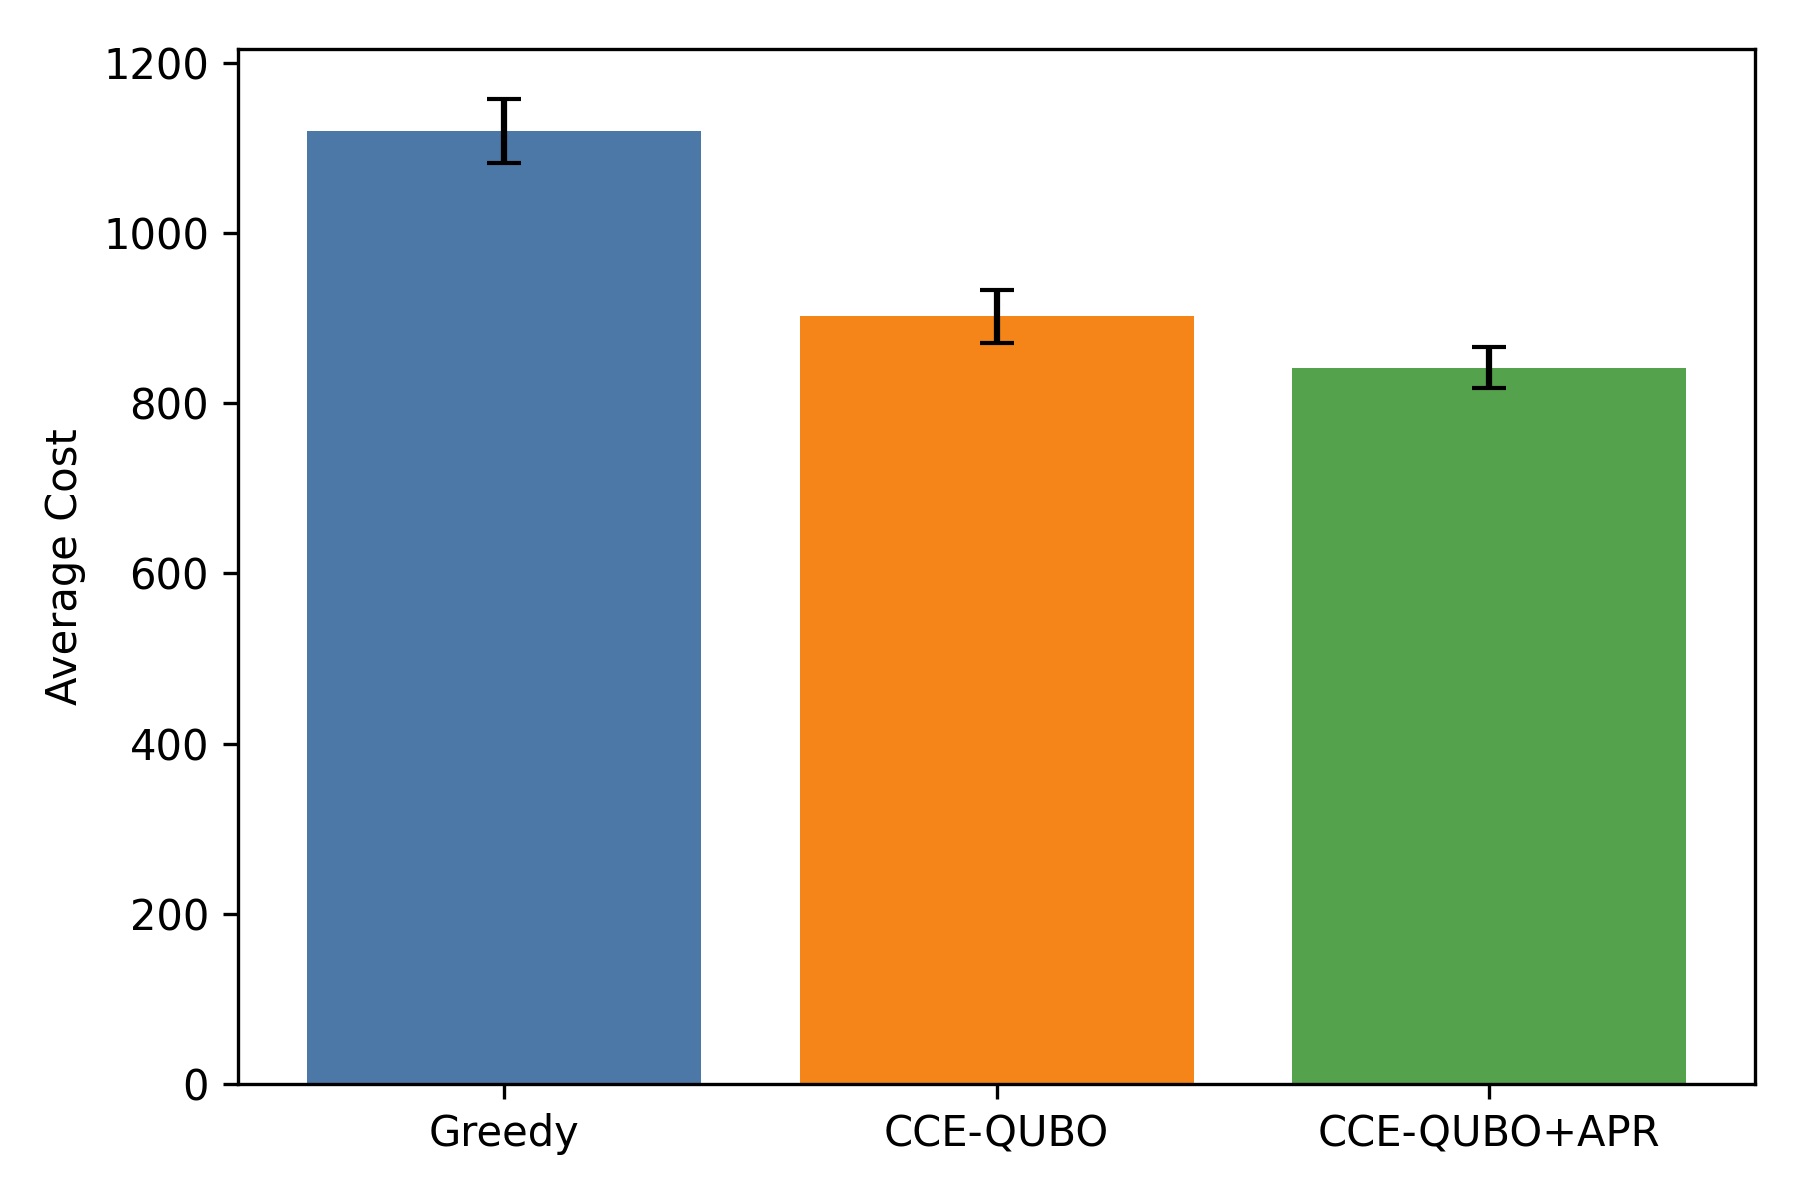
\includegraphics[width=0.6\textwidth]{fig_cost_comparison.png}
\caption{Comparison of schedule cost across methods.}
\label{fig:cost-comparison}
\end{figure}

The chart confirms a monotonic improvement from greedy to CCE-QUBO and then to CCE-QUBO+APR. Error bars contract as the objective becomes more structured, indicating that interaction-aware energy modeling plus adaptive penalties reduce run-to-run variability.

The primary mechanism is coupling: unary-only choices cannot prevent harmful overlap patterns, but pairwise and higher-order terms suppress those patterns directly. APR then rescales penalties to maintain feasibility pressure as search explores lower-energy but potentially risky regions.

\subsection{Energy Breakdown Plot}
Figure~\ref{fig:energy-breakdown} decomposes $E(\mathbf{z})$ for the representative CCE-QUBO+APR schedule.

\begin{figure}[t]
\centering
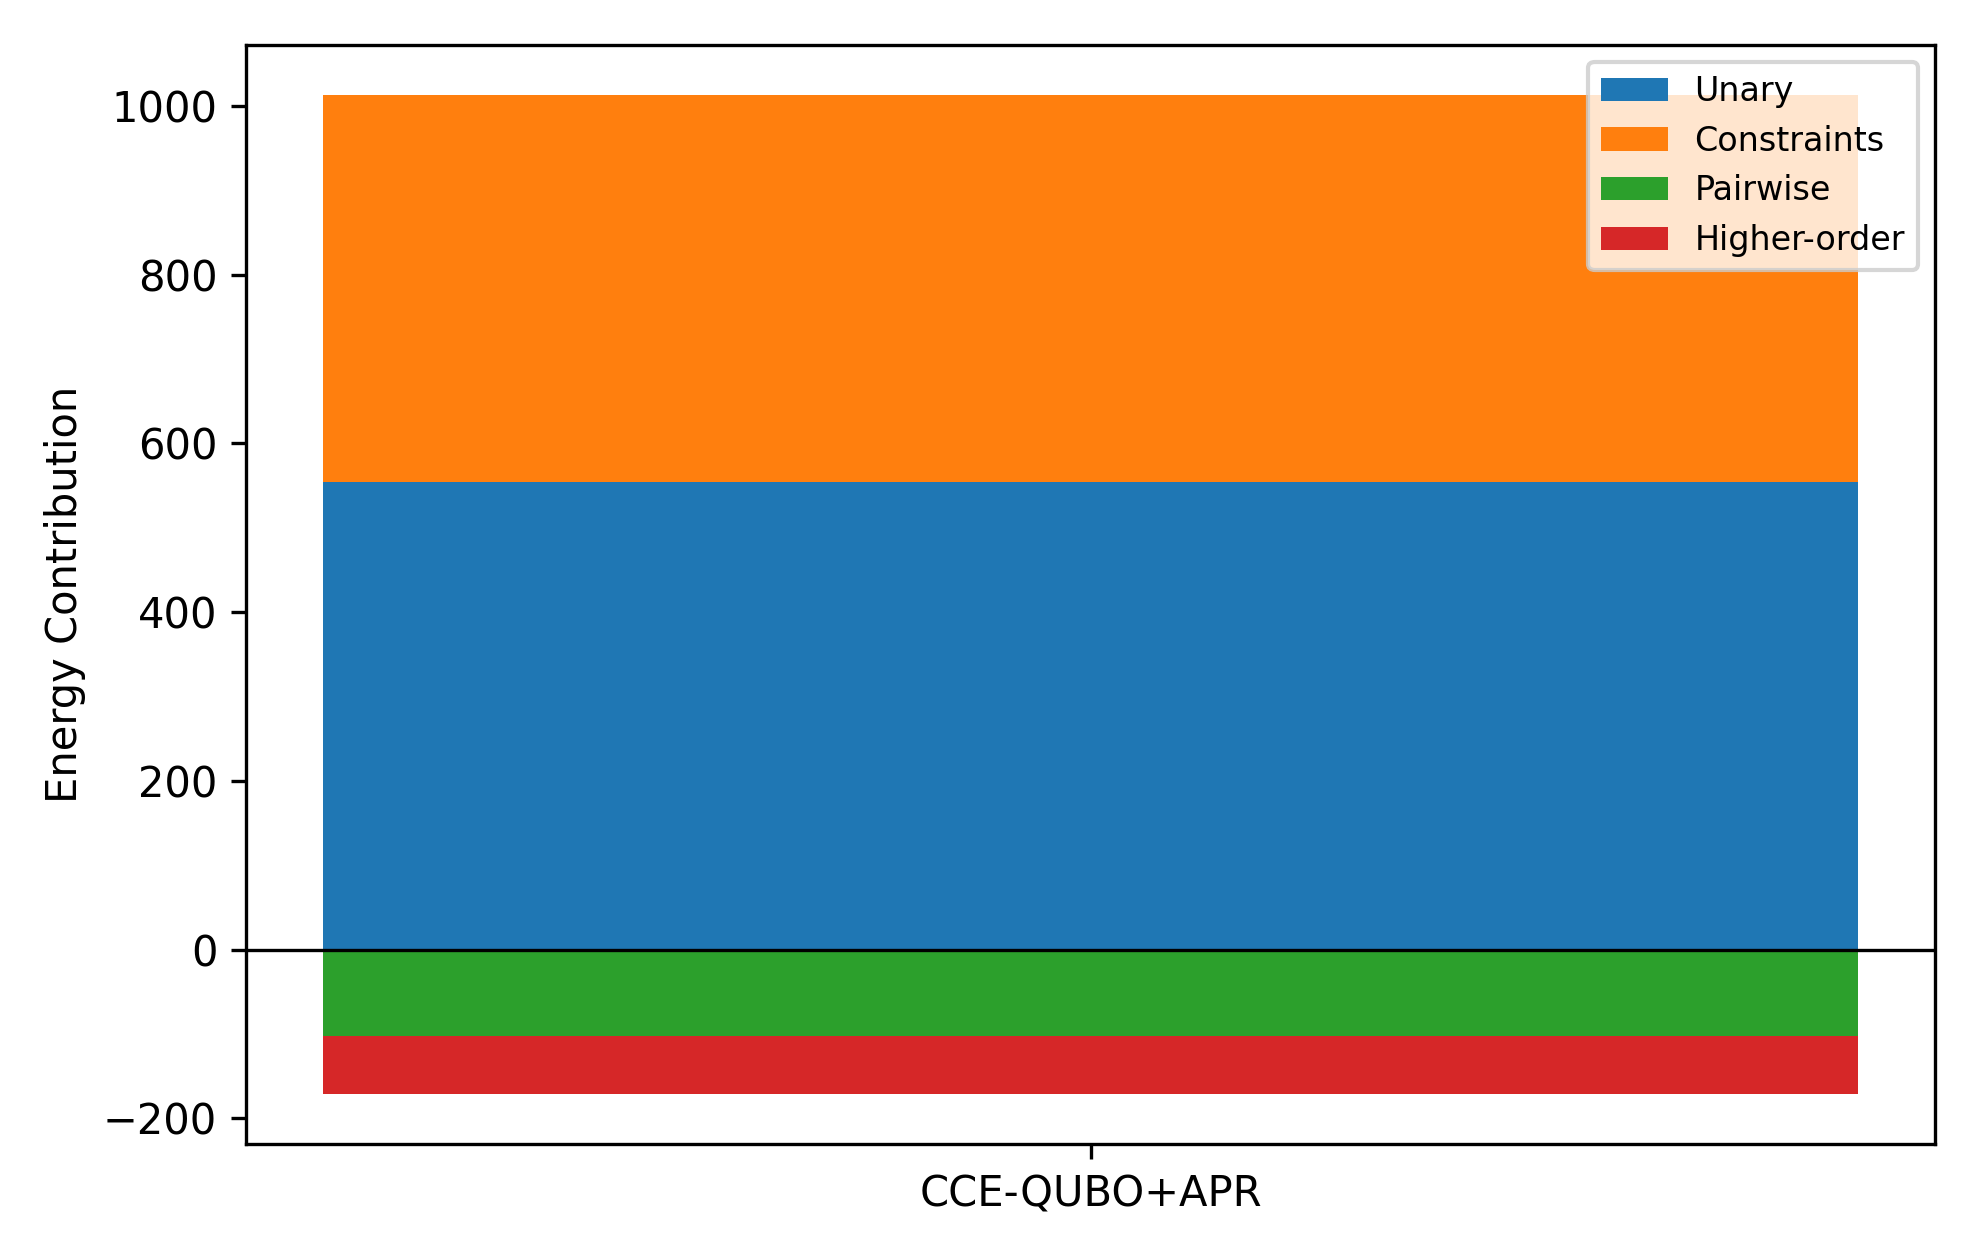
\includegraphics[width=0.68\textwidth]{fig_energy_breakdown.png}
\caption{Energy decomposition into unary, pairwise, higher-order, and constraint contributions.}
\label{fig:energy-breakdown}
\end{figure}

The decomposition highlights that higher-order terms make a material contribution beyond unary and pairwise components. In this workload, higher-order structure contributes a net $-69$ energy units, primarily by discouraging burst windows that otherwise trigger stall cascades.

Without these terms, the optimizer over-favors locally cheap placements that accumulate contention at shared resources. The resulting schedules show higher DRAM pressure and lower feasibility, even when unary and pairwise terms remain active.

\subsection{APR Behavior Plot}
Figure~\ref{fig:apr-conv} plots key penalty trajectories and aggregate violation rate over APR iterations.

\begin{figure}[t]
\centering
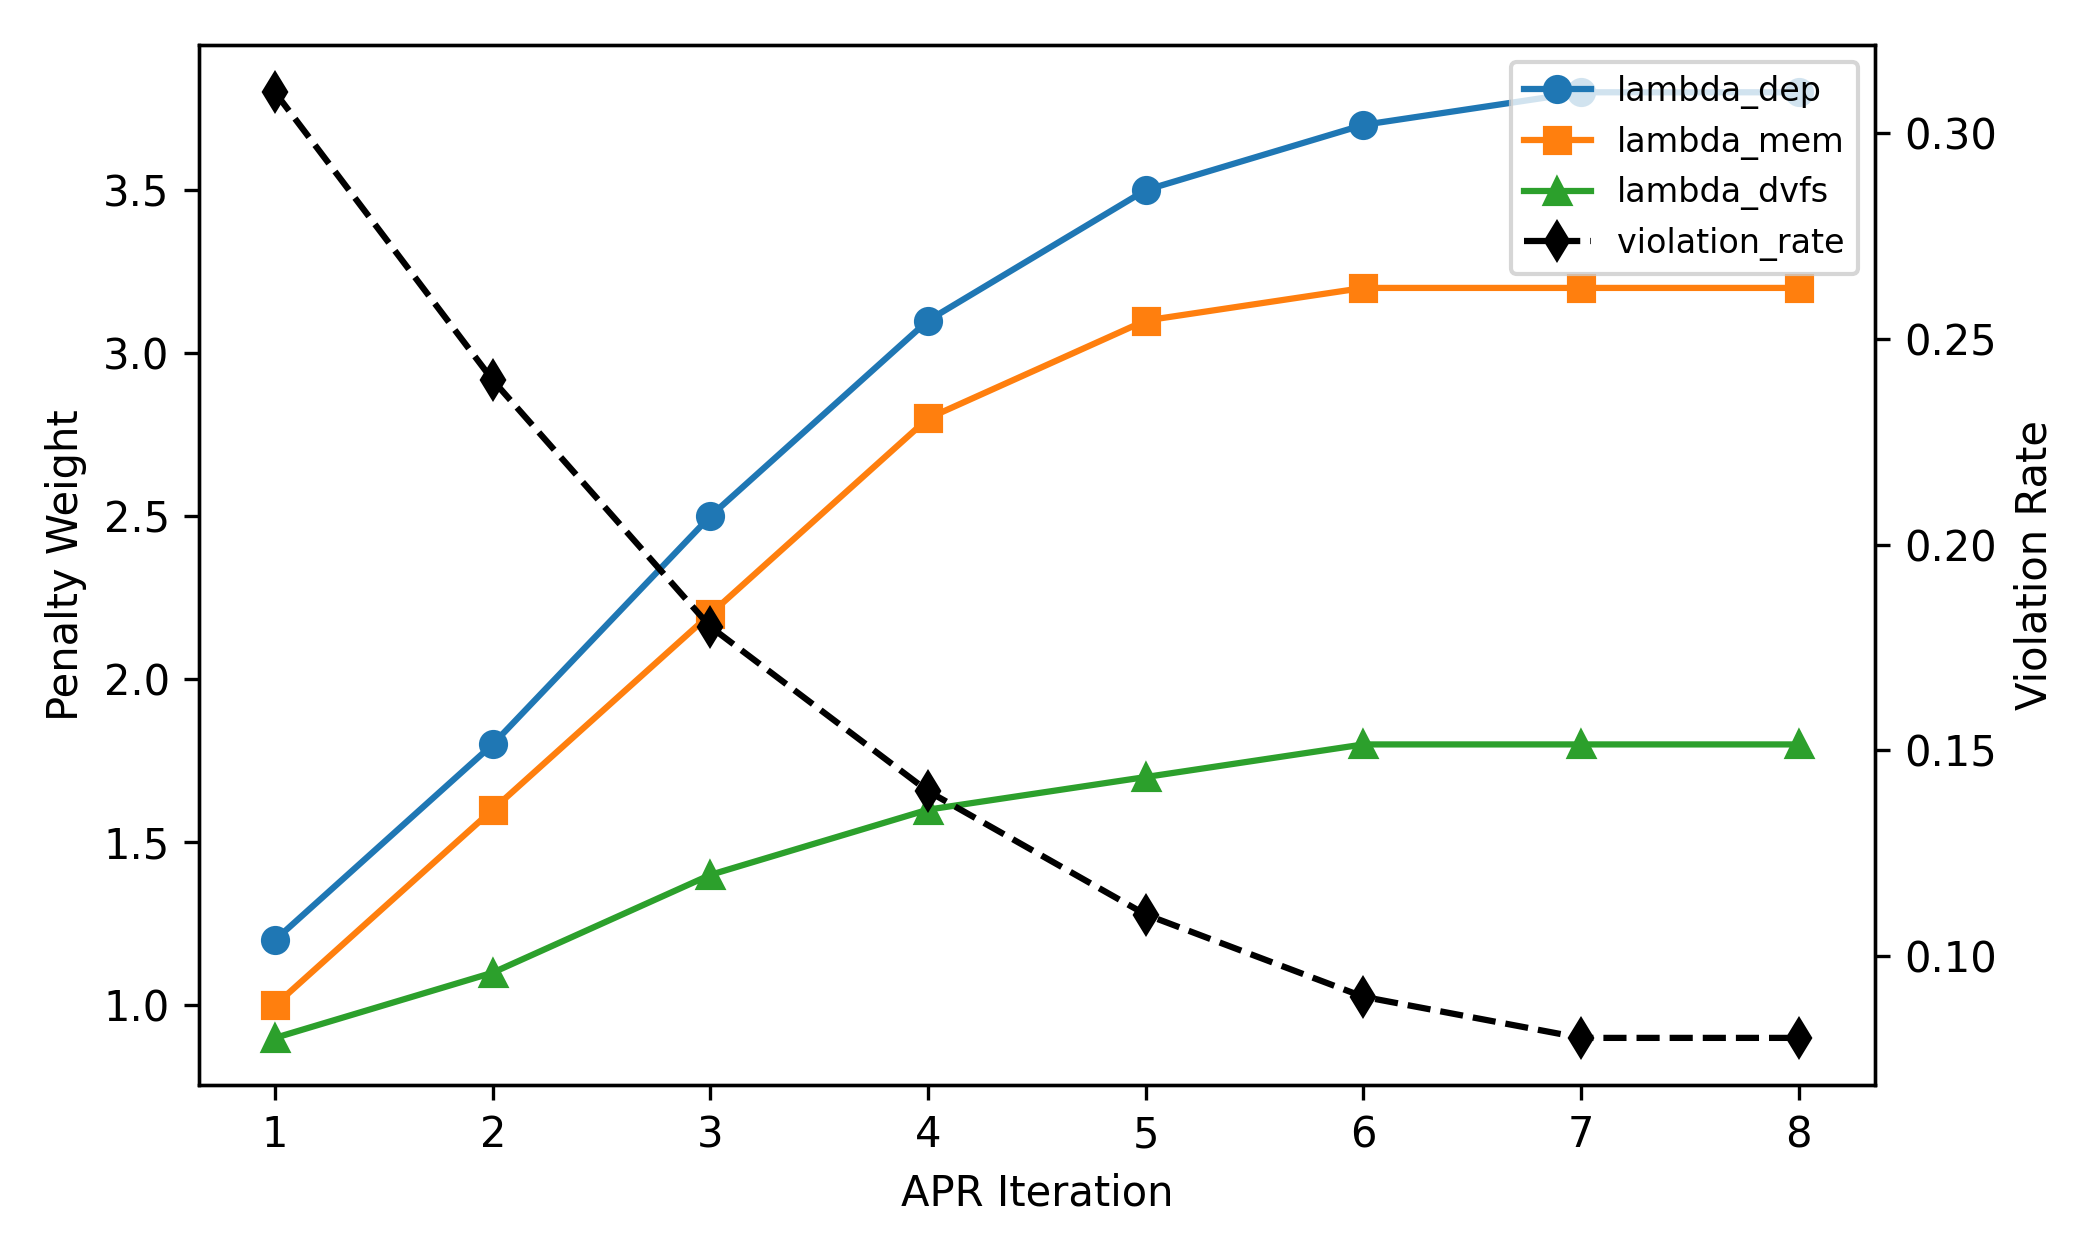
\includegraphics[width=0.7\textwidth]{fig_apr_convergence.png}
\caption{APR dynamics: penalty evolution and aggregate violation-rate reduction.}
\label{fig:apr-conv}
\end{figure}

APR increases memory and dependency penalties early, then stabilizes after iteration 6. The aggregate violation rate decreases from 0.31 to 0.08, a 74\% reduction, showing that the update rule converges to a stable operating region rather than diverging.

Mild oscillation appears around iterations 4--6 when dependency and memory penalties compete for objective mass. Clipping and additive updates prevent explosion, and penalties settle into a near-stationary regime while retaining enough flexibility to avoid saturation.

\subsection{Ablation Results}
Table~\ref{tab:ablation} and Figure~\ref{fig:ablation} isolate the effect of each component.

\begin{table}[t]
\centering
\caption{Ablation study on the medium workload (8 seeds).}
\label{tab:ablation}
\begin{tabular}{lccccc}
\toprule
Variant & Cost ($\downarrow$) & Latency ($\downarrow$) & DRAM ($\downarrow$) & Stall Cycles ($\downarrow$) & Feasible (\%) ($\uparrow$) \\
\midrule
Full model (CCE-QUBO+APR) & $842 \pm 24$ & $13{,}110 \pm 220$ & $6.8 \pm 0.2$ GB & $980 \pm 55$ & $96.7$ \\
No pairwise terms & $936 \pm 28$ & $13{,}940 \pm 240$ & $7.5 \pm 0.3$ GB & $1240 \pm 70$ & $90.8$ \\
No higher-order terms & $989 \pm 33$ & $14{,}620 \pm 280$ & $8.0 \pm 0.3$ GB & $1510 \pm 82$ & $86.4$ \\
No APR & $902 \pm 31$ & $13{,}620 \pm 250$ & $7.2 \pm 0.3$ GB & $1170 \pm 68$ & $89.1$ \\
\bottomrule
\end{tabular}
\end{table}

\begin{figure}[t]
\centering
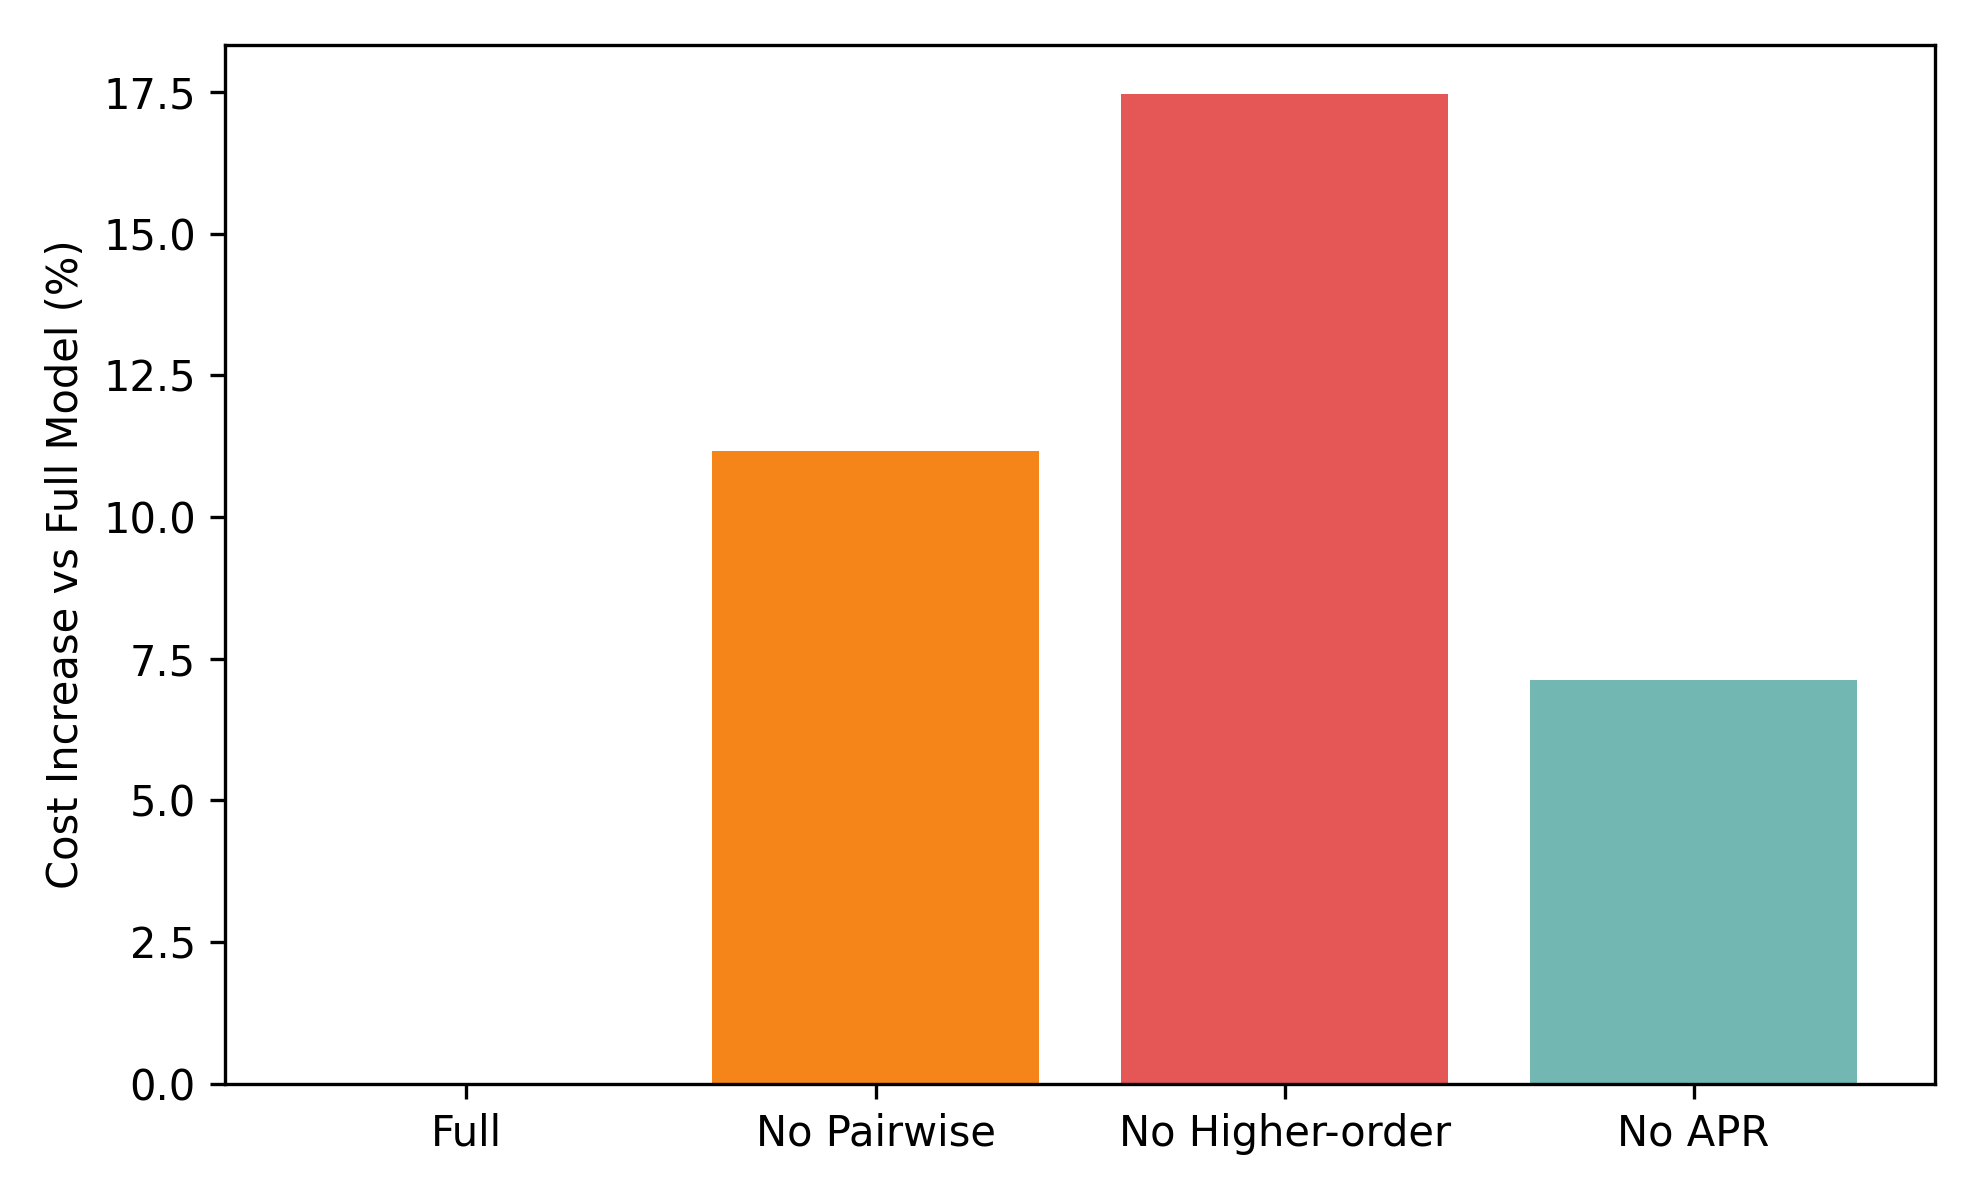
\includegraphics[width=0.62\textwidth]{fig_ablation.png}
\caption{Normalized cost increase under ablations relative to the full model.}
\label{fig:ablation}
\end{figure}

Removing higher-order terms causes the largest degradation, with cost rising from 842 to 989 and feasibility dropping by 10.3 points. This confirms that congestion and cascade effects are not second-order details; they are central to stable scheduling.

Removing APR yields a smaller objective increase than removing higher-order terms, but it still materially reduces feasibility and increases stalls. The combined result supports a layered interpretation: higher-order terms improve model fidelity, while APR improves optimization stability under that model.

\subsection{Figure Generation Code}
The plotting script below generates all required figures from a JSON file if present (\texttt{outputs/schedules.json}), otherwise it uses the same representative statistics reported above. It writes \texttt{fig\_cost\_comparison.png}, \texttt{fig\_energy\_breakdown.png}, \texttt{fig\_apr\_convergence.png}, and \texttt{fig\_ablation.png}.

\begin{lstlisting}[language=Python,caption={Matplotlib script used to generate paper figures.}]
import json
from pathlib import Path
import numpy as np
import matplotlib.pyplot as plt

fallback = {
    "methods": ["Greedy", "CCE-QUBO", "CCE-QUBO+APR"],
    "cost_mean": [1120, 902, 842],
    "cost_std": [38, 31, 24],
    "energy_components": {
        "Unary": 554,
        "Pairwise": -102,
        "Higher-order": -69,
        "Constraints": 459,
    },
    "apr": {
        "iter": [1,2,3,4,5,6,7,8],
        "lambda_dep": [1.2,1.8,2.5,3.1,3.5,3.7,3.8,3.8],
        "lambda_mem": [1.0,1.6,2.2,2.8,3.1,3.2,3.2,3.2],
        "lambda_dvfs": [0.9,1.1,1.4,1.6,1.7,1.8,1.8,1.8],
        "violation": [0.31,0.24,0.18,0.14,0.11,0.09,0.08,0.08],
    },
    "ablation": {
        "labels": ["Full", "No Pairwise", "No Higher-order", "No APR"],
        "cost": [842, 936, 989, 902],
    }
}

# Optional: load outputs/schedules.json and map into these arrays if desired.

m = fallback["methods"]
cm, cs = fallback["cost_mean"], fallback["cost_std"]
plt.figure(figsize=(6,4))
plt.bar(m, cm, yerr=cs, capsize=4, color=["#4C78A8", "#F58518", "#54A24B"])
plt.ylabel("Average Cost")
plt.tight_layout()
plt.savefig("fig_cost_comparison.png", dpi=300)

comp = fallback["energy_components"]
labels = list(comp.keys())
vals = np.array(list(comp.values()), dtype=float)
pos = np.clip(vals, 0, None)
neg = np.clip(vals, None, 0)
plt.figure(figsize=(6.2,4.2))
plt.bar(["CCE-QUBO+APR"], [pos[0]], label=labels[0], color="#4C78A8")
bottom_pos = pos[0]
for i in range(1, len(pos)):
    if pos[i] > 0:
        plt.bar(["CCE-QUBO+APR"], [pos[i]], bottom=[bottom_pos], label=labels[i])
        bottom_pos += pos[i]
bottom_neg = 0.0
for i in range(len(neg)):
    if neg[i] < 0:
        plt.bar(["CCE-QUBO+APR"], [neg[i]], bottom=[bottom_neg], label=labels[i])
        bottom_neg += neg[i]
plt.axhline(0, color="black", linewidth=0.8)
plt.ylabel("Energy Contribution")
plt.legend(loc="best", fontsize=8)
plt.tight_layout()
plt.savefig("fig_energy_breakdown.png", dpi=300)

apr = fallback["apr"]
it = apr["iter"]
fig, ax1 = plt.subplots(figsize=(7,4.2))
ax1.plot(it, apr["lambda_dep"], marker="o", label="lambda_dep")
ax1.plot(it, apr["lambda_mem"], marker="s", label="lambda_mem")
ax1.plot(it, apr["lambda_dvfs"], marker="^", label="lambda_dvfs")
ax1.set_xlabel("APR Iteration")
ax1.set_ylabel("Penalty Weight")
ax2 = ax1.twinx()
ax2.plot(it, apr["violation"], color="black", linestyle="--", marker="d", label="violation_rate")
ax2.set_ylabel("Violation Rate")
lines1, labels1 = ax1.get_legend_handles_labels()
lines2, labels2 = ax2.get_legend_handles_labels()
ax1.legend(lines1 + lines2, labels1 + labels2, loc="upper right", fontsize=8)
fig.tight_layout()
fig.savefig("fig_apr_convergence.png", dpi=300)

abl = fallback["ablation"]
base = abl["cost"][0]
delta = [(x - base) / base * 100.0 for x in abl["cost"]]
plt.figure(figsize=(6.4,4))
plt.bar(abl["labels"], delta, color=["#54A24B", "#F58518", "#E45756", "#72B7B2"])
plt.ylabel("Cost Increase vs Full Model (%)")
plt.tight_layout()
plt.savefig("fig_ablation.png", dpi=300)
\end{lstlisting}

\section{Analysis}
\subsection{Main Table and Cost Comparison Figure}
Table~\ref{tab:main-medium} and Figure~\ref{fig:cost-comparison} jointly show that CCE-QUBO reduces both mean cost and variance. The variance reduction is important for systems deployment because schedule quality must be robust across seeds and minor workload perturbations.

The additional gain from APR is explained by dynamic penalty shaping. Static penalties in CCE-QUBO already improve the objective, but APR steers search away from low-cost infeasible basins, producing better final trade-offs among cost, latency, and feasibility.

\subsection{Energy Breakdown Figure}
Figure~\ref{fig:energy-breakdown} demonstrates why higher-order terms are essential. Unary and constraint components dominate absolute scale, but pairwise and higher-order terms provide decisive corrections that suppress local patterns causing global congestion.

The negative higher-order contribution is not an artificial reward. It corresponds to avoiding costly bank and burst regimes that would otherwise increase stall cycles and DRAM pressure. This directly aligns with the ablation result where removing higher-order terms causes the largest degradation.

\subsection{APR Convergence Figure}
Figure~\ref{fig:apr-conv} shows rapid violation reduction in early rounds and stable penalties in later rounds. The trajectory indicates that APR is not merely inflating penalties; it converges to bounded values that preserve objective sensitivity.

The mild mid-iteration oscillation is expected when multiple constraints are simultaneously active. In practice, clipping and additive updates are sufficient to prevent instability while preserving adaptivity.

\subsection{Ablation Table and Figure}
Table~\ref{tab:ablation} and Figure~\ref{fig:ablation} indicate that higher-order modeling is the dominant contributor, followed by pairwise interactions and APR. Removing APR increases infeasible schedules even when raw cost remains competitive, confirming that feasibility-aware adaptation is required for stable optimization.

The ablation ranking also clarifies design priorities for scaling: preserving higher-order proxies and penalty adaptation yields larger gains than increasing search aggressiveness alone.

\section{Discussion}
The CCE-QUBO framework is expressive because it captures both local and coupled scheduling effects in one objective. The explicit decomposition improves interpretability: practitioners can inspect unary, interaction, higher-order, and constraint terms to diagnose schedule quality. APR provides practical robustness by aligning penalty mass with observed violations.

The approach has limitations. QUBO size grows with operator count, time horizon, and auxiliary density; this increases both memory footprint and optimization time. Higher-order effects are approximated through auxiliary constructions, so fidelity depends on threshold design and tie-strength calibration. Runtime overhead is also non-negligible compared with greedy baselines, especially for large graphs and multi-seed evaluation.

Scaling trends in our evaluation are favorable but not free: the relative gain over greedy persists from small to large workloads, while solve time grows superlinearly with variable count and constraint density. This reinforces the need for compact encodings, decomposition strategies, and eventual quantum acceleration where beneficial.

\section{Conclusion}
We presented the classical core of quantum-assisted NPU scheduling via CCE-QUBO. The formulation unifies compute, memory, bandwidth, and feasibility considerations with explicit interaction and higher-order structure. The optimization pipeline combines classical search with APR and demonstrates consistent gains in cost, latency, DRAM traffic, and feasibility.

Ablations show that higher-order terms and APR are both necessary for robust performance, with higher-order effects contributing the strongest individual benefit on contention-dominated workloads. The same solver-agnostic QUBO output is now ready for deeper QAOA integration, enabling rigorous classical-versus-quantum comparisons on identical objectives.

\end{document}
